%%%%%%%%%%%%%%%%%%don't forget if needed %%%%%%%%%%%%%%%%%%%%%
%\section[toc version]{title version%
%              \sectionmark{head version}}
%\sectionmark{head version}
%%%%%%%%%%%%%%%%%%%%%%%%%%%%%%%%%%%%%%%%%%%%%%%%%%%%%%%%%%%%%%
\def\titcourt{A finite-element toolbox}
\def\titlong{A finite-element toolbox for the simulation of phase-change systems with natural convection}
%%%%%%%%%%%%%%%%%%%%%%%%%%%%%%%%%%%%%%%%%%%%%%%%%%%%%%%%%%%%%%%%
\chapter[\titlong]{\titlong%
              \chaptermark{\titcourt}}
\chaptermark{\titcourt}
\label{chap-ToolBox}
%%%%%%%%%%%%%%%%%%%%%%%%%%%%%%%%%%%%%%%%%%%%%%%%%%%%%%%%%%%%%%%%
%%%%%%%%%%%%%%%%%%%%%%%%%%%%%%%%%%%%%%%%%%%%%%%%%%%%%%%%%%%%%%%%


\section{A finite-element toolbox for the simulation of phase-change systems with natural convection}\label{sec-desc-prog}

The methods described previously were implemented in a 2D toolbox based on \ff software.
In this section we first describe the architecture of the programs and the organisation of files.
Then we focus on the list of input parameters and the structure of output files.
%
\begin{figure}[!h]
	\begin{center}
		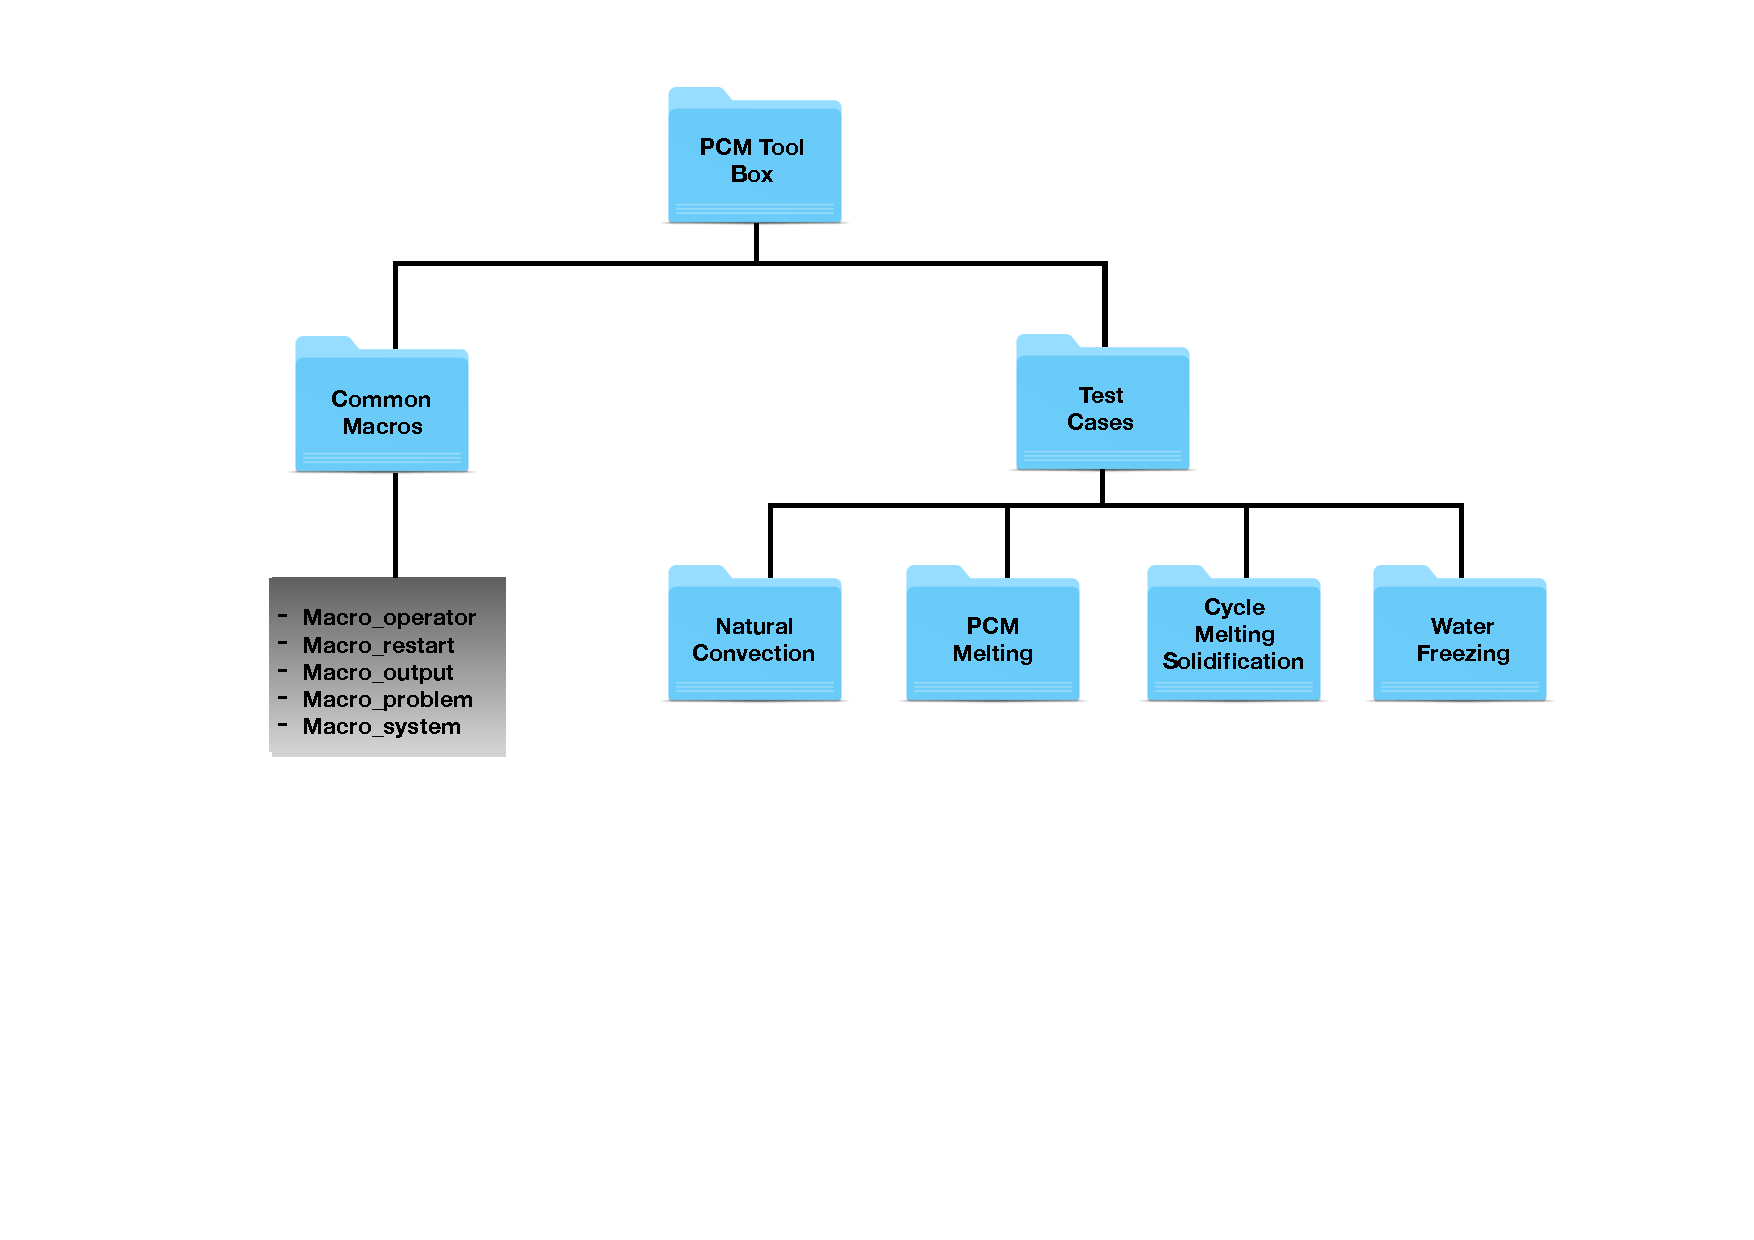
\includegraphics[width=0.9\textwidth]{\figpath/Fig_cap_2/FOLDER_arbor_3}
	\end{center}
	\caption{Folder tree structure of the FreeFem++ toolbox to solve phase change problems. Test cases and common macros are separated into two folders.}
	\label{fig-folder-tree}
\end{figure}

\section{Program architecture}
Figure \ref{fig-folder-tree} gives a schematic overview of the content of the toolbox. All files are provided in a directory called \texttt{PCM-Toolbox}.  Many detailed comments are included in the programs, with direct link to the mathematical expressions used in the paper. The used \ff syntax was intentionally kept at a low level of technicality and supplemented with detailed comments when specific more technical syntax was used.

This directory is organized as follows:
\begin{enumerate}
   \item The directory \texttt{Common-Macros} contains five files:\\
$\bullet$ {\em Macro$\_$operator.idp} includes macros and functions defining mathematical operators,\\
$\bullet$ {\em Macro$\_$problem.idp}: macros defining the variational formulation of the problem,\\
$\bullet$ {\em Macro$\_$restart.idp}: macros used to start a new simulation from a saved field,\\
$\bullet$ {\em Macro$\_$output.idp}: macros used to save the solution with different formats,\\
$\bullet$ {\em Macro$\_$system.idp}: macros identifying the OS and defining specific OS-commands.

   \item The directory \texttt{Test-Cases}  contains four subdirectories, each of them defining one of the following applications:\\
    $\bullet$  natural convection of air or water in a differentially heated square cavity, \\
    $\bullet$  melting of a PCM stored in containers of different shapes,\\
    $\bullet$  melting followed by solidification of a rectangular PCM,\\
    $\bullet$  freezing of pure water in a square cavity.\\
   Each subdirectory contains  three files: {\em NEWTON$\_$\$case.edp} is the main \ff script file, $param_\_phys.inc$ defines the physical parameters and $param_\_num.inc$ the numerical parameters. For example, to run the natural convection case of air in a square cavity, the user can use the following command in a terminal window:
  \texttt{FreeFem++ NEWTON$\_$stat$\_$natconv.edp}.\\
  The folder structure of each test case is illustrated in Figure \ref{fig-case-folder}.
  The obtained solutions are saved in the folder \texttt{OUTPUT/Data}. Depending on the output format selected by the user,  data files are generated in specific folders for being visualized with: Tecplot, Paraview, Gnuplot or Medit. We also provide in the folder \texttt{Figures} ready-made layouts for these visualisation softwares. The user can thus obtain the figures from this paper using  newly generated data. More details about the output structure are given below.
\end{enumerate}

\begin{figure}[!h]
	\begin{center}
		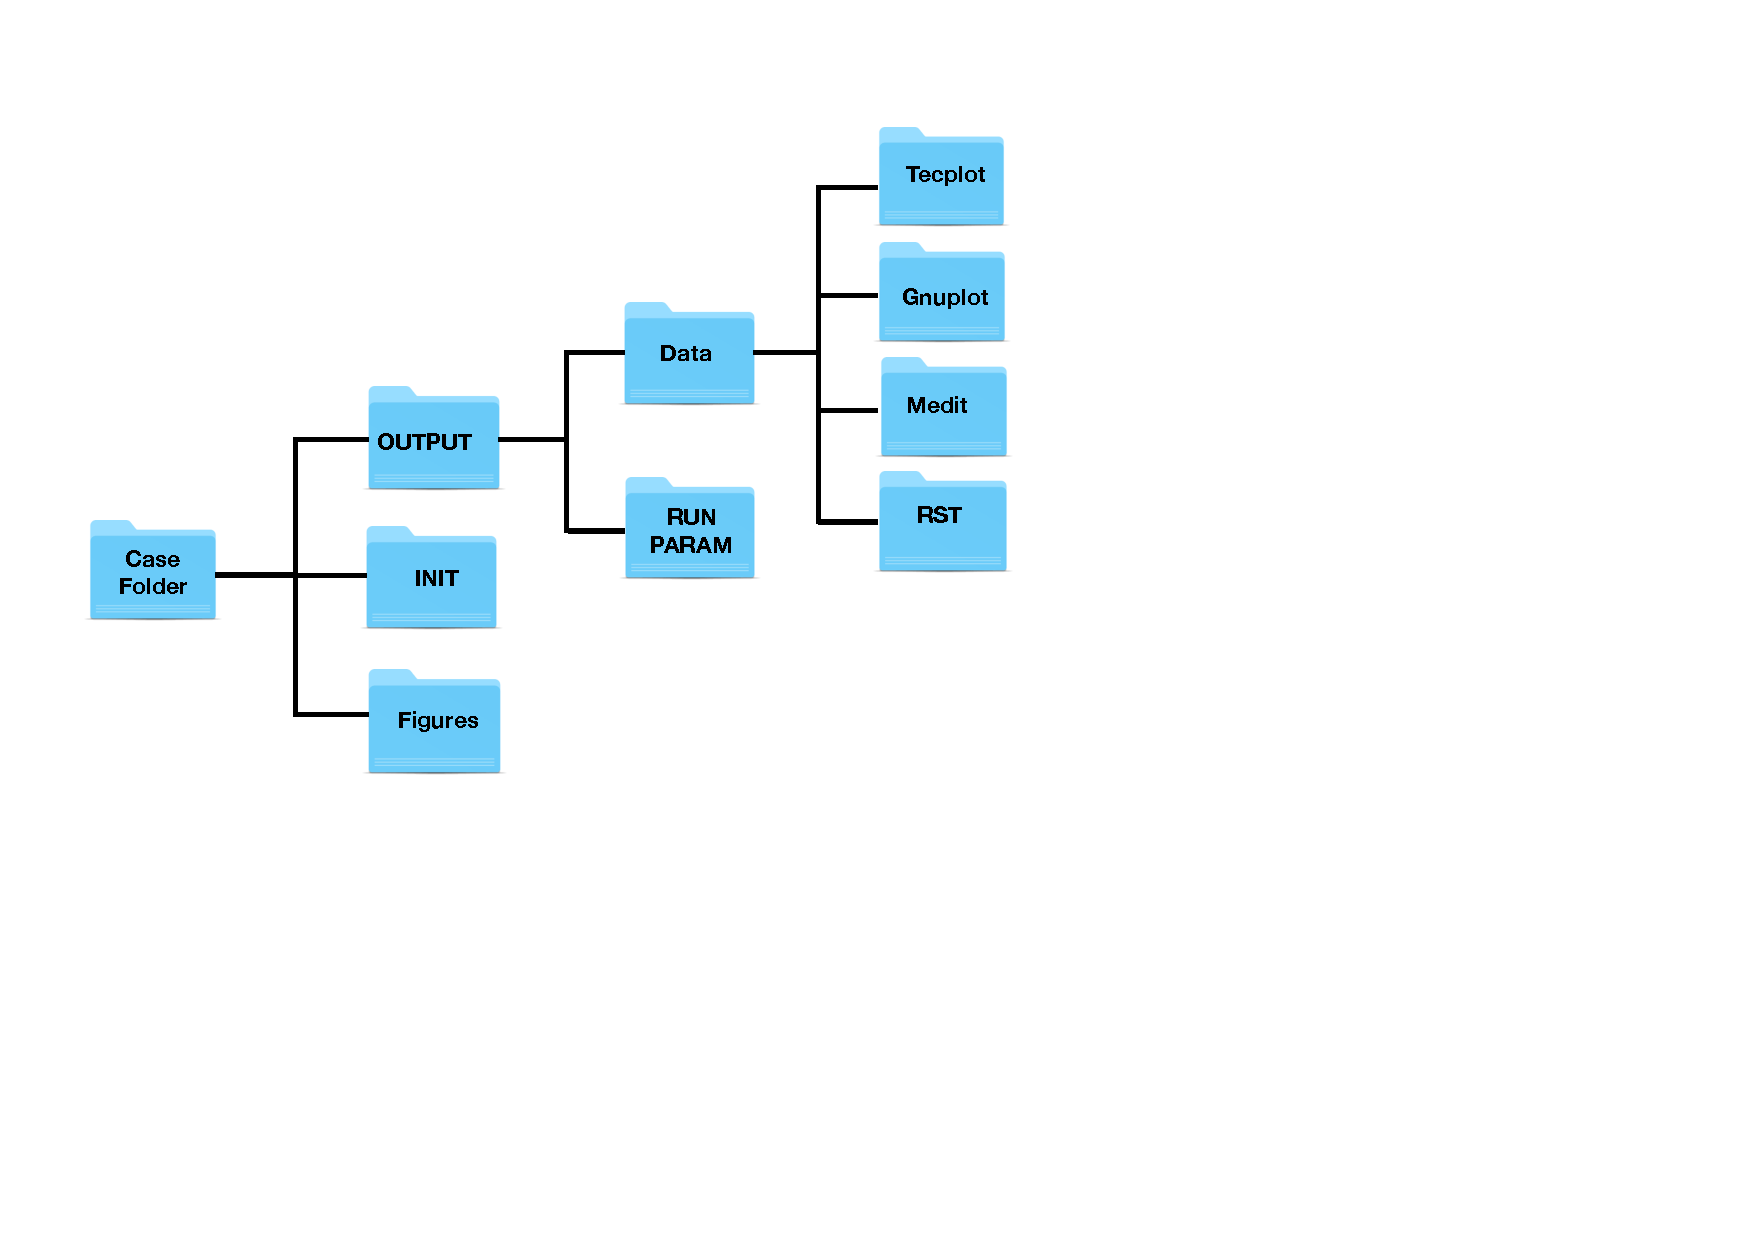
\includegraphics[width=0.7\textwidth]{\figpath/Fig_cap_2/figsCPC_02}
	\end{center}
	\caption{Structure of each Test-case folder. 
	}
	\label{fig-case-folder}
\end{figure}

\section{Input parameters}

Physical parameters and parameters related to the run are separated into two files.\\
{\bf (1)} The file $param_\_phys.inc$ contains the physical descriptions of the problem:
\begin{itemize}
   \item {\bf typeT}: is the finite-element type for the temperature, with possible values \texttt{P2} or \texttt{P1},
   \item {\bf Torder}: is the accuracy order of the time integration scheme, with possible values $1$ (Euler scheme) or $2$ (Gear scheme),
   \item {\bf scalAdim}: defines the characteristic scales of the problem, see (\ref{eq-adim}). Possible values 1, 2 or 3 correspond to the following choice of the characteristic scales \citep{dan-2014-JCP}:
   \begin{eqnarray} \label{eq-scal1}
    (1) &:&  V_\vref^{(1)} = \frac{\nu_l}{H} \Longrightarrow \ds t_\vref^{(1)} = \frac{H^2}{\nu_l}  \Longrightarrow \Rey=1,\\
      \label{eq-scal2}
     (2) &:& V_\vref^{(2)} = \frac{\alpha}{H} \Longrightarrow \ds t_\vref^{(2)} = t_\vref^{(1)} \Prd  \Longrightarrow \Rey =1/\Prd,\\
      \label{eq-scal3}
     (3) &:& V_\vref^{(3)} = \frac{\nu_l}{H} \sqrt{\frac{\Ray}{\Prd}} \Longrightarrow \ds t_\vref^{(3)} = t_\vref^{(1)} \sqrt{\frac{\Prd}{\Ray}}       \Longrightarrow \Rey = \sqrt{\frac{\Ray}{\Prd}},
\end{eqnarray}
   \item {\bf x$_l$, x$_r$, y$_l$, y$_r$}: are the values defining the dimensions of the cavity $[x_l,x_r]\times[y_l,y_r]$,
   \item {\bf Pr, Ra, Ste}: are the  Prandtl, Rayleigh and Stefan numbers, see (\ref{eq-Rayleigh}) and (\ref{eq-RePr}),
   \item {\bf T$_{hot}$, T$_{cold}$}: are  dimensionless temperatures according to (\ref{eq-adim}),
   \item{\bf bcu$_1$, bcu$_2$, bcT}: are macros defining the velocity (u) and the temperature (T) boundary conditions.
   \item {\bf epsi}: is the half width $\varepsilon$ of the mushy region. \underline{Default value} = $0.01$,
   \item {\bf dt}: is the dimensionless time step,
   \item {\bf t$_{max}$}: is the dimensionless final time,
   \item {\bf Parameters for regularization functions}: \\
 The parameters of the hyperbolic-tangent function (\ref{eq-smooth}) used to regularize discontinuous functions are set by default as follows:
 \end{itemize}
    \begin{table}[!ht]
    \centering
    \begin{tabular}{*{8}{c}}
     & { f$_{s}$} & {f$_{l}$} & {a$_s$} & {$\theta_s$} & R$_s$ & {$\CKC$} & {b} \\
       \toprule
       {\it Enthalpy} & 0 & 1/Ste & 1 & 0.01 & 0.01  & - & - \\
       \midrule
       {\it Carman - Kozeny} & 0 & 1 & 1 & 0.01 & 0.01  & 10$^6$ & 10$^{-7}$ \\
          \midrule
       {\it Conductivity (water)} & 1 & 2.26/0.578 & 1 & $\theta_f$ & 0.015 & - & - \\
       \bottomrule
     \end{tabular}
    \label{tab-constant}
    \end{table}
   \begin{itemize} 
    \item {\bf rho(T) and Drho(T)}: (water cases only) define  the density and its derivative as functions of the temperature, following the model
\citep{Gebhart1977}:\\
 
    \begin{table}[!ht]
    \centering
    \begin{tabular}{*{4}{c}}
    	\multicolumn{4}{c}{
      $\rho(T) = \rho_m (1 - \omega | T - T_m |^q),$}\\	\hline
    $\rho_m$ [kg/m$^3$]  & $\omega$ [$^o$C$^{-q}$] & q & $T_m$  [$^o$C] \\
       \toprule
            $999.972$ & $9.2793 \cdot 10^{-6}$ & $1.894816$ & $4.0293$ \\
       \bottomrule
     \end{tabular}
    \label{tab-rho}
    \end{table}
    \item {\bf f$_B$(T), df$_B$(T)}: define the buoyancy force and its derivative.
    \end{itemize}

\noindent {\bf (2)} The file {\em param$\_$num.inc} contains the parameters controlling the run.\\
{\bf Restart parameters:}
\begin{itemize}
   \item {\bf Nsave}: the solution is saved every $N\!save$ time steps in the \texttt{Data} folder (see Figure \ref{fig-case-folder}). The temperature and the velocity fields are saved in \texttt{Tecplot} and \texttt{Medit} folders, while the liquid fraction, the Nusselt number, and the accumulated heat input are saved in the \texttt{Gnuplot} folder.
   \item {\bf Nrestart}: restart files (mesh and solution) are saved every $N\!restart$ time steps. Solutions at current and previous iterations, the CPU time, the accumulated heat input $Q_0$, and the time step $dt$ are saved in the folder \texttt{RST}.
   \item {\bf Ncondt}: allows the user to stop the run and save the solution properly. The file \texttt{OUTPUT/zz.condt} is read every $N\!condt$ time steps: if the user replaces the value "0" in this file by "1" the run is stopped. This is a simple solution for a clean stop of the job by the user. \underline{Default value} = $20$.
   \item {\bf Nremesh}: the mesh is adapted every $N\!remesh$ iterations. If this parameter is set to "1" the mesh is adapted every time step.
   \item {\bf IFrestart}: is a boolean controlling the set up of the initial field. \\
  $I\!Frestart = 0$, the  initial condition is built in the code for each test case. For the PCM melting cases, the PCM is initially motionless at isothermal temperature. 
  	To set-up a smooth initial field, a few time steps (with very small $\delta t$) are computed by increasing progressively the boundary temperature at the hot wall and the Rayleigh number (by continuation).  Outputs are saved in  \texttt{OUTPUT/Data-RST-0}.\\
   $I\!Frestart > 0$, (positive integer values) the solution field previously computed at iteration $I\!Frestart$ is loaded from the folder \texttt{OUTPUT/Data-RST-filenameRST/RST}, with \texttt{filenameRST} a variable selecting the restart folder. \\
   $I\!Frestart < 0$, (negative integer values), the same principle for loading a solution is used, but from the folder \texttt{INIT}  (see Figure \ref{fig-case-folder}). The solution fields stored in this folder could come from different previous calculations (\eg a steady state solution or, for the water, the natural convection field before freezing).
\end{itemize}

{\bf Newton parameters:}
\begin{itemize}
   \item {\bf epsconv}: is the value of  the stopping criterion for steady cases,
   \item {\bf gamma}: is the penalty parameter in  (\ref{eq-time-disc1}). \underline{Default value} = $10^{-7}$,
   \item {\bf tolNewton}: is the Newton tolerance $\xi_N$ (see (\ref{eq-Newton-algo})). \underline{Default value} = $10^{-6}$,
   \item {\bf newtonMax}: limits the maximum number of iterations in  the Newton algorithm (\ref{eq-Newton-algo}). \underline{Default value} = $50$,
  % \Blue{\item {\bf c$_1$, c$_2$, c$_3$}: \Red{(-- why not negative $a_2$ ?? si c'est trop compliqu� de changer, il faut le laisser tel quel --$>$ } \Blue{C'est modifi� en a$_2$ n�gatif maintenant dans le code)--}  are the coefficients of the time integration scheme: c$_1 =1/$dt, c$_2 = -1/$dt, c$_3 = 0$ correspond to the first order backward Euler scheme and c$_1 =1.5/$dt, c$_2 = -2/$dt, and c$_3 = 0.5/$dt to the second order Gear scheme.}
\end{itemize}
{\bf Mesh parameters:}
\begin{itemize}
   \item {\bf nbseg}: is  the number of segments for the discretisation along the $x$ and $y$ directions,
   \item {\bf errh}: is the interpolation error level. \underline{Default value} = $0.02$,
   \item {\bf hmin, hmax}: are the minimum and maximum edge size, respectively,
   \item {\bf adaptratio}: is the ratio for a prescribed smoothing of the metric. For a value less than $1.1$ no smoothing is done. \underline{Default value} = $1.5$,
   \item {\bf nbvx}: is the maximum number of vertices allowed in the mesh generator. \underline{Default value} = $50000$.
\end{itemize}

\noindent {\bf Output parameters:}
   \begin{itemize}
      \item {\bf dircase}: is the name of the output folder,
      \item {\bf fcase}: is the prefix-name for ouput files.
      \item {\bf Tecplot, Medit, Gnu}: correspond to the name of the visualisation software to be used; the format of the outputs written in \texttt{OUTPUT/Data} (see Figure \ref{fig-case-folder}) is accordingly set.  The files from the Tecplot folder can be easily read  also with Paraview.
   \end{itemize}
   
\section{Outputs}
When a computation starts, the \texttt{OUTPUT} directory is created (see Figure \ref{fig-case-folder})).
It contains two folders storing the output data and the echo of the run parameters.
The folder \texttt{Data} contains four subdirectories with different output format files of the computed solution. File names are created using  the prefix defined by the parameter {\bf fcase}, the current iteration and the current dimensionless time $t$. 
Solution files can be visualized using either Tecplot or any other CFD Visualization tools (Paraview, Visit, etc.). 
Moreover, {\em .gmsh}  (mesh) and {\em .rst} (fields) files are generated in the folder \texttt{RST} to enable restarts of the computation. Note that the folder \texttt{FFglut} contains  \ff scripts that re-read and visualize the RST-files to facilitate the selection of a restart field.  
An {\em .echo} file with a summary of the main parameters, informations on the run and the names of the output files is saved in the folder \texttt{RUNPARAM}.  This directory additionally contains a copy of the {\em .inc} parameter files, allowing an easy identification of each case and preparing an eventual rerun of the same case.

